%%%%%%%%%%%%%%%%%%%%%%%%%%%%%%%%%%%%%%%%%%%%%%%%%%%%%
%												    %
%	REDES DE COMPUTADORES						 %
%												    %
%	Novembro 2015								    %
%												    %
%	Angela Cardodo e Bruno Madeira					%
%   											    %	
%%%%%%%%%%%%%%%%%%%%%%%%%%%%%%%%%%%%%%%%%%%%%%%%%%%%%

\documentclass[11pt,a4paper,reqno]{report}
\linespread{1.2}


\usepackage{rotating}
\usepackage{tikz}
\usepackage[active]{srcltx}    
\usepackage{graphicx}
\usepackage{amsthm,amsfonts,amsmath,amssymb,indentfirst,mathrsfs,amscd}
\usepackage[mathscr]{eucal}
\usepackage{tensor}
\usepackage[utf8x]{inputenc}
\usepackage[portuges]{babel}
\usepackage[T1]{fontenc}
\usepackage{enumitem}
\setlist{nolistsep}
\usepackage{comment} 
\usepackage{tikz}
\usepackage[numbers,square, comma, sort&compress]{natbib}
\usepackage[nottoc,numbib]{tocbibind}
%\numberwithin{figure}{section}
\numberwithin{equation}{section}
\usepackage{scalefnt}
\usepackage[top=1cm, bottom=2cm, left=2cm, right=2cm]{geometry}
%\usepackage{tweaklist}
%\renewcommand{\itemhook}{\setlength{\topsep}{0pt}%
%	\setlength{\itemsep}{0pt}}
%\renewcommand{\enumhook}{\setlength{\topsep}{0pt}%
%	\setlength{\itemsep}{0pt}}
%\usepackage[colorlinks]{hyperref}
\usepackage{MnSymbol}
%\usepackage[pdfpagelabels,pagebackref,hypertexnames=true,plainpages=false,naturalnames]{hyperref}
\usepackage[naturalnames]{hyperref}
\usepackage{enumitem}
\usepackage{titling}
\newcommand{\subtitle}[1]{%
	\posttitle{%
	\par\end{center}
	\begin{center}\large#1\end{center}
	\vskip0.5em}%
}
\newcommand{\HRule}{\rule{\linewidth}{0.5mm}}
\usepackage{caption}
\usepackage{etoolbox}% http://ctan.org/pkg/etoolbox
\usepackage{complexity}

\usepackage[official]{eurosym}

\def\Cpp{C\raisebox{0.5ex}{\tiny\textbf{++}}}

\makeatletter
\def\@makechapterhead#1{%
  %%%%\vspace*{50\p@}% %%% removed!
  {\parindent \z@ \raggedright \normalfont
    \ifnum \c@secnumdepth >\m@ne
        \huge\bfseries \@chapapp\space \thechapter
        \par\nobreak
        \vskip 20\p@
    \fi
    \interlinepenalty\@M
    \Huge \bfseries #1\par\nobreak
    \vskip 40\p@
  }}
\def\@makeschapterhead#1{%
  %%%%%\vspace*{50\p@}% %%% removed!
  {\parindent \z@ \raggedright
    \normalfont
    \interlinepenalty\@M
    \Huge \bfseries  #1\par\nobreak
    \vskip 40\p@
  }}
\makeatother

\usepackage[toc,page]{appendix}

\addto\captionsportuges{%
  \renewcommand\appendixname{Anexo}
  \renewcommand\appendixpagename{Anexos}
}

\addto\captionsportuges{%
  \renewcommand\abstractname{\huge Sumário}  
}

\usepackage{verbatim}
\usepackage{color}
\definecolor{darkgray}{rgb}{0.41, 0.41, 0.41}
\definecolor{green}{rgb}{0.0, 0.5, 0.0}
\usepackage{listings}
\lstset{language=C++, 
    basicstyle=\linespread{0.8}\ttfamily,
    keywordstyle=\color{blue}\ttfamily,
	showstringspaces=false,
    stringstyle=\color{red}\ttfamily,
    commentstyle=\color{green}\ttfamily,
	identifierstyle=\color{darkgray}\ttfamily,
    morecomment=[l][\color{magenta}]{\#},
	tabsize=4,
    breaklines=true
}

\begin{document}



\begin{titlepage}
\begin{center}
 
\vspace*{3cm}

{\Large Redes de Computadores}\\[2cm]

% Title
{\Huge \bfseries Protocolo de Liga\c{c}\~ao de Dados \\[1cm]}

% Author
{\large \^Angela Cardoso e Bruno Madeira}\\[2cm]


\includegraphics[width=10cm]{feup_logo.jpg}\\[2cm]


% Bottom of the page
{\large \today}

\end{center}
\end{titlepage}


%%%%%%%%%%%
% SUMARIO %
%%%%%%%%%%%
\begin{abstract}
	
Este relatório tem como objectivo reportar o segundo trabalho prático relativo a Redes de Computadores da Licenciatura com Mestrado em Engenharia Informátia e Computação. 


\end{abstract}

\tableofcontents

%%%%%%%%%%%%%%
% INTRODUCAO %
%%%%%%%%%%%%%%
\chapter{Introdução}


	
%%%%%%%%%%%%%%%
% APLICAÇÂO %
%%%%%%%%%%%%%%%
\chapter{Aplicação}

A aplicação deve receber informação no formato estabelecido no guião para ser realizado o parsing desta e estabelecida a conexão. Não foram considerados utilizadores anónimos como é referido no rfc???? em ????. Relaizando o parsing fica guardado numa estrutura o nome de utilizador, password, nome do host, caminho ate ao ficheiro e o nome do ficheiro.

Uma vez realizado o parsing tenta-se obter o ip do destino e cria-se uma ligação tcp para a porta 21 do servidor a fim de enviar os comandos para pedir a recepção do ficheiro.

São usadas duas sockets na aplicação, uma aberta inicialmente para enviar comandos ao servidor e outra aberta mais tarde pare a transmissão de dados. 
TODO

%%%%%%%%%%%%%%%%%%%%
% LABS REALIZADOS%
%%%%%%%%%%%%%%%%%%%%
\chapter{Experiências}
...
\section{Experiência 1 - Configurar uma Rede IP}

Nesta experiência criou-se uma LAN com o tux1 e o tux4 na mesma rede e configurados os seus endereços ip. Usando o comando ping na etapa 7, pudemos verificar o envio de um comando ARP em broadcast pelo tux1 que procurava o endereço físico do tux4, necessário ao protocolo ethernet usado para poder comunicar dentro de uma mesma rede local. Seguidamente vericou-se a resposta do tux4 e foi realizado o ping com sucesso.

Atentando aos pacotes do wireshark podesse verificar o que os pacotes ARP são identificáveis pelo cabeçalho Ethernet x0806 e os IP pelo x0800. As mensagens de ping, do tipo ICMP, podem ser identificadas pelo cabeçalho IP x01 cabeçalho Ethernet correspondente ao IP.

TODO loopback interface e frame length

\section{Experiência 2 - Implementar 2 LANs num switch}
...
\section{Experiência 3 - Configurar um Router em Linux}
...
\section{Experiência 4 - Configurar um Router Comercial e Implementar NAT}
...
\section{Experiência 5 - DNS}

\section{Experiência 6 -Conexões TCP}

\section{Experiência 7 }

%%%%%%%%%%%%%%%
% VALORIZACAO %
%%%%%%%%%%%%%%%
\chapter{Elementos de valorização}


%%%%%%%%%%%%%%
% CONCLUSOES %
%%%%%%%%%%%%%%
\chapter{Conclusões}


%%%%%%%%%%%%%%%%
% BIBLIOGRAPHY %
%%%%%%%%%%%%%%%%


\begin{appendices}

%%%%%%%%%%%%%%%%%%%%%%%%%%%
% APENDICE - VARIAS %
%%%%%%%%%%%%%%%%%%%%%%%%%%%
\chapter{Enderaços MAC}

\begin{itemize} 
\item TUX1: 00:0f:fe:8c:af:71
\item TUX2: 00:21:5a:5a:7d:9c
\item TUX3: 00:21:5a:61:2f:4e
\item TUX4: 00:21:5a:c5:61:bb
\end{itemize}

\chapter{Wireshark}

\section{Ex1}
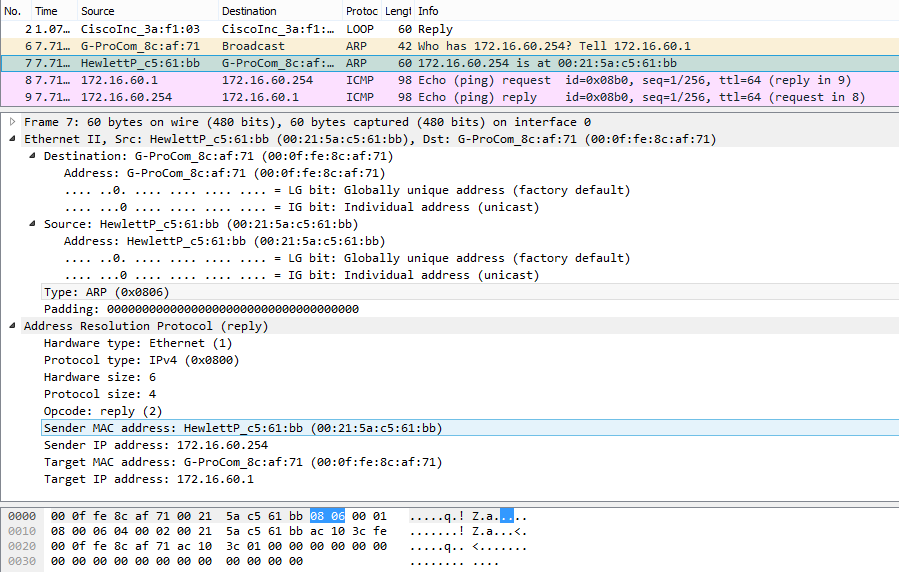
\includegraphics[width=20cm]{ex1_arp.png}
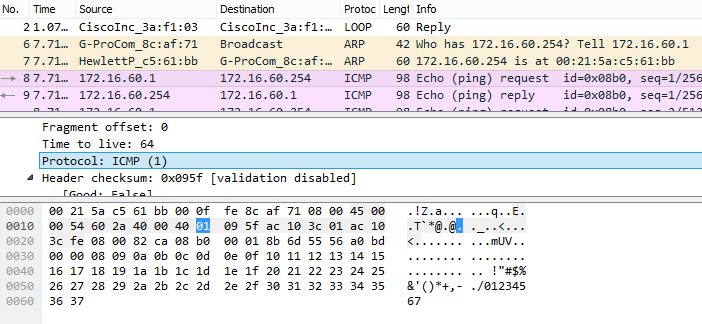
\includegraphics[width=20cm]{ex1_icmp.png}

%%%%%%%%%%%%%%%%%%%%%%%%%%%
% APENDICE - CODIGO FONTE %
%%%%%%%%%%%%%%%%%%%%%%%%%%%
\chapter{Código Fonte}

\end{appendices}

\end{document}
